% !TeX spellcheck = en_GB
\section{Theoretical Background}
In the following some physical concepts needed for the understanding of this experiment are explained.
%\subsection{Physical Concepts}
\subsection{Colour Centres}




Diamond structure is a well know and studies in crystallography, It lattice consist in a cubic structure based on 8 Carbon atoms, two tetrahedrally bonded atoms in each primitive. The diamond lattice is basically two face-centred cubic lattices, being the face centres (FCC) atom on one cell the vertices of the other. Since there are two  identical atoms per unit cell, there is no absorption of photon in the IR-region, This mean that a pure diamond can not have fluorescence properties (in first order) but this properties can be achieve with changes due impurities in the structure. This properties are call Colour centres.

Colour centres (CC) are a kind of point defects in crystal structures which contain a electron that absorbs light of certain wavelengths. This basic defect in the regular spacing of atoms within a solid that absorbs visible light of a particular colour, lending a characteristic colour to the solid. \\

There are more then 100 luminescent defects in diamond. Another name that is knowns is F-centre (German Farbe, “colour”), results from the absence of a negatively charged ion from a particular point in an ionic solid. This vacancy, which acts like a positively charged particle, attracts and traps an electron, and their combination constitutes an Colour-centre.  One of the most abundant and also  studied one is the  Nitrogen related defects, or Nitrogen-Vacancy centres (NV) , because  nitrogen is a prominent impurity in the material, In next section we will talk in more detail about its properties.


\subsection{NV-Centres in Diamonds}
\label{sec:nvcentres}
 The NV-centres are a defect or impurities in the diamond structure, where two carbon atom in the secondary fcc are replaced , one by a nitrogen atom and the second one by a  vacant. The single substitutional nitrogen has an infra-red mode of vibration. Nitrogen aggregates are, pairs of neighbouring substitutional atoms, the nitrogen aggregates, and it neighbours that lead to different combination ( eighteen total usually labelled according to corresponding Miller indices) in the lattices that have distinct infra-red spectra. In the next figure, the Fist Fcc lattice of the diamond is shown and in the conduce structure one of the carbons was replaced by the $N$. NV-centre can exist in two charge states, the neutral $NV^{0}$ state and the negatively charged $NV^{-}$ state that have different energy levels and alloud transition.
 
The most interesting properties of the NV centres is its abortion and emission fluorescence at red region, property fundamental that will be studied in this experiment, and is mostly due to physical effects by the magnetic moment. A simplified quantum structure of the NV centre can be seen in the fig .... where the ground stade and exited stade are contructed by triplet stades with a distance of 1.945 eV in between, here calles $^{3}A_{2}$ and $^{3}E$  respectivelly. The main radiative connection between the ground state and the excited state is due to the zero phonon line (ZPL). For the negatively charged NV center, this transition contributes to a wavelength of $\lambda_{zpl} = 637\,\mathrm{nm}$ and has a lifetime of 10-30 ns.(To observe the ZPL, a simple absortion emition proces was done with a 519nm laser was done, identifin this peak at... .) 
An aditional proces from the exited stade is a nonradiative emission into the metastable singlet state $\left|s\right\rangle$ . This can either occur from the state $\left| e,ms\right\rangle$, in a weak non-radiative decay.

\begin{figure}
	\centering
	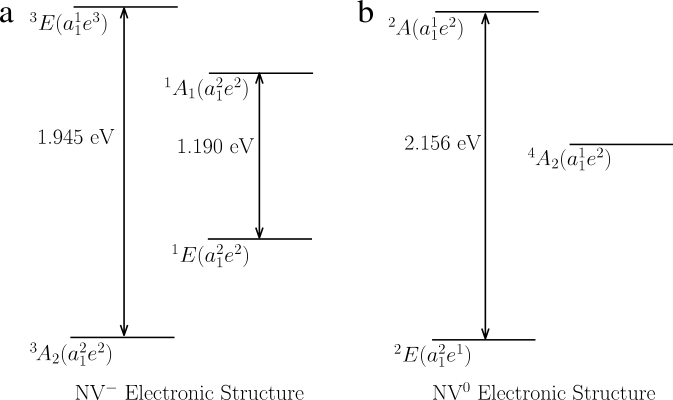
\includegraphics[width=0.5\textwidth]{../figures/nv-centre.png}
	\caption{Electronic structure of (a) $NV^-$ and (b) NV$^0$ centres \cite{doherty}}
	\label{fig:nvcentres}
\end{figure}


The wide properties on $NV^{-}$ centres have made this research gain popularity in wide range of application as temperature sensing \cite{neumann_high-precision_2013}, pressure sensing \cite{doherty_electronic_2014} and even biological applications \cite{mcguinness_quantum_2011}. The NV- centre presents a well detectable zero phonon (ZPL), in literature at 637 nm  and has a lifetime of 10-30 ns as shown in the next figure \ref{jeske_stimulated_2017}, typically it is excited with $\lambda_{exc}=532nm$, while it can be excited in a broad band below. In simple word the ZPL is presented as it name says, when an emission or absorption between two states occurs with out extra phonon in the process. When a round sated and an exited sated counts with several process available the transition between the two levels can be with the exact energy between the two or also with $\pm phonons$ to the other possible degraded states of the lattice, in this cases one or more phonon are release, making the colour centres to a have a broad spectra of emission \ref{sild_zero-phonon_1988}.
On the other hand  the fluorescence ranges also over a broad range and only a few percent of the photons are emitted into the ZPL; the major part emits into vibrational side-bands in the range of 630 to 800 nm \cite{doherty} and  Non-radiative decay to $\left\|s\right\rangle$ can also occur, which, in turn, has a lifetime of about 250 ns \cite{schirhagl_nitrogen-vacancy_2014}

%\subsection{Experimental Methods}
\subsection{Optically Detected Magnetic Resonance}

Optical detected magneto resonance or ODMR, is  a  double  resonance  technique  which  combines  optical
measurements, in our case the fluorescence of the $nv^{-}$, with  electron  spin  resonance  spectroscopy.  After  the  first
triplet-state ODMR experiment in zero magnetic field reported  in 1968 \cite{schmidt_optical_1967}, the  number  of double resonance studies on excited triplet states grew rapidly.  The ground state of a typical organic molecule is a
singlet state, and absorption of light leads to excited singlet states. The unpairing of the electron spins is possible only if
there is some degree of spin-orbit coupling, If this happens, then the molecule undergoes intersystem crossing (ISC)  and  becomes  a  triplet  state. After an excited molecule crosses into a triplet state, it may remain there a long time because the de-excitation is
spin-forbidden \cite{carbonera_optically_2009}.
As we refer in the last section our $NV^{-}$ in the ground state $\left| g \right\rangle $ at $m=0$ using a wipe of microwaves with a centre of frequency exactly at energy gap to $\left\| g,m=\pm1\right\rangle $, this leads to two important consequence. First that our system is now a triplet state and so the emission at m=0 are forbidden now from the excite state $\left\| e,m=0\right\rangle $ and second that this allow to a major percentage of the non radiative emission to be present from $\left\| s\right\rangle $ to the ground state. This detuning in the microwave can be calculated on base the Hamiltonians of each levels and is equal to \cite{schirhagl_nitrogen-vacancy_2014}:\\
\begin{equation}
\omega_{mw}=(E_{\left|g,m=0\right\rangle}-E_{\left|g,m=\pm 1\right\rangle}/ \hslash = 2π X 2870MHz 
\end{equation}
Where $\omega_{ws}$ is the frequency centres of the microwave and E is the energy of each level.

The spin properties of NV defects can also be used for magnetic field measurements \cite{sage_optical_2013}. In the presence of a static magnetic field, the degeneracy of the NV defect states is lifted by the Zeeman effect.  It leads to the appearance of two resonance lines in the electron spin resonance spectrum. The frequency of the splitting resonances is then directly related to the amplitude of the applied magnetic field B NV along the NV defect axis  \cite{lesik_engineering_2015}. The spatial resolution of a single NV scanning probe magnetometer is fundamentally limited by the electron spin wave function, which is in the Angstrom range. NV center application in high sensitivity magnetometer a single NV defect is integrated onto the tip of an atomic force microscope and used as an atomic-sized magnetic field sensor under ambient conditions. \cite{zhou_scanning_2017}.
Using the magnetic field $B$ the the magnetic moment $\mu$ will look as:\\
\begin{align}
\mu&=\dfrac{\mu_{b}}{\hslash}*g_{s}*s \\
\mu&=\gamma*s
\end{align}
Where $\mu_{b}$ is the Bohr´s magnetron and $g_{s}\simeq 2$, $s$ and $\gamma$ are the g-factor, spin and the gyromagnetic ratio for the free electron respectively. \cite{meschede_gerthsen_2015} At $B\neq 0$ and $\gamma=2\pi*2.8GHZ$ the energy gaps between the $m_{s}=1$ and $-1$ looks like:
\begin{align}
	\Delta E&=(E_{0}-\hslash \gamma B_{0}*cos\alpha)-(E_{0}-\hslash \gamma \\	
	\Delta E&=2*\hslash \gamma B_{0}*cos\alpha
\end{align}
Where $\alpha $ is the angle between the magnetic field and magnetic moment. The original resonance is split symmetrically into two magnetic ones, which are detuned around the centre frequency.
\begin{equation}
	\omega=\gamma B_{0}*cos\alpha
\end{equation}
This mean that our frequency centre is not only sensitive to the amplitude of the magnetic field, but also to the orientation between the crystal and the external field. Furthermore, the isolation of the NV center intrinsic influences includes stability of this measurement, providing a sensitive tool to detect magnetic fields \cite{meschede_gerthsen_2015}.

